\documentclass[10pt,a4paper]{article}

\usepackage[a4paper,margin=1in]{geometry}
\usepackage[T1]{fontenc}
\usepackage{lmodern}
\usepackage{microtype}
\usepackage{graphicx}
\usepackage{booktabs}
\usepackage{amsmath}
\usepackage{amssymb}
\usepackage{url}
\usepackage{hyperref}
\usepackage{caption}
\usepackage{subcaption}
\usepackage{enumitem}
\usepackage{multirow}
\usepackage{authblk}

\graphicspath{{figures/}}
\hypersetup{colorlinks=true,linkcolor=black,urlcolor=blue,citecolor=black}

\title{\bfseries A Unified RGB Pipeline for Face Anti-Spoofing:\\
Combined-Dataset Training of AttackNet v2.2 on Replay-Attack and 3DMAD}

\author[1]{Author Name}
\affil[1]{Department of Computer Science, University Name}

\date{\today}

\begin{document}
\maketitle

\begin{abstract}
Face anti-spoofing models trained on a single benchmark routinely achieve
near-zero error within their own test set yet fail badly when
transferred to a different attack family or capture device. We argue
that the dominant cost in building a generalising classifier is not
architectural but \emph{logistical}: each public benchmark ships in a
different format, with a different annotation schema, and a different
notion of ``split''. We present a unified RGB-only preprocessing
pipeline that collapses two structurally different datasets ---
Replay-Attack (2D photo and video presentations) and 3DMAD (3D mask
attacks) --- into a single CSV manifest of $77{,}296$ identically-shaped
$256{\times}256$ face crops, and we train AttackNet v2.2, a compact
$8.4$M-parameter residual CNN, from scratch on their union.
Within-dataset test ACER is below $0.5\%$ on both benchmarks.
Cross-dataset evaluation reveals a sharp \emph{asymmetry}:
Replay $\rightarrow$ 3DMAD transfers at $2.8\%$ frame ACER (HTER
$8.8\%$ after devel calibration), whereas 3DMAD $\rightarrow$ Replay
collapses to $38.8\%$ frame ACER (HTER $22.7\%$). We interpret this
as evidence that single-dataset models learn camera- and
protocol-specific shortcuts rather than a general notion of liveness.
A further probe on the held-out CSMAD corpus (silicone mask attacks,
Intel RealSense SR300) deepens this conclusion: the combined model
achieves a devel-calibrated HTER of $0.58$ and a ROC-AUC of
$\mathbf{0.40}$ --- a \emph{ranking inversion}. The model scores
genuine CSMAD faces as more attack-like than actual silicon masks,
because the SR300 sensor characteristics push real faces into the
high-attack region of the learned feature space. An AUC below $0.5$,
confirmed after threshold calibration, is the empirical signature of
this inversion and shows that camera-hardware change alone --- without
any change in attack family --- is sufficient to break a PAD model
worse than random.
\end{abstract}

\section{Introduction}
\label{sec:intro}

A face presentation attack detector (PAD) sees the same input as a face
verification system --- a photograph of a face --- and must decide
whether the photograph depicts a live human or a presentation
artefact: a printed photograph, a video replayed on a phone screen,
or a silicone mask. The literature reports two seemingly inconsistent
facts: modern CNN-based detectors saturate the standard public
benchmarks (Replay-Attack \cite{anjos2011replay}, 3DMAD
\cite{erdogmus20143dmad}, CSMAD \cite{bhattacharjee2018csmad})
at sub-$1\%$ error; yet PAD models that are deployed without
retraining on the target distribution fail far more often than these
numbers would suggest. The cross-dataset gap is now well-documented
and is a direct consequence of training a classifier on a single,
narrow capture protocol.

This paper does not propose a new architecture. Instead we make a
deliberately mundane methodological argument: the most actionable lever
for closing the cross-dataset gap, before any architectural change,
is to \emph{merge the public benchmarks at the data layer} and train a
single model on their union. The benefit per unit of effort is large,
because (i) the public benchmarks have systematically different
weaknesses and (ii) a uniform manifest is a one-time engineering cost
that all subsequent experiments amortise.

Concretely, our contributions are:

\begin{enumerate}[leftmargin=*,topsep=2pt,itemsep=2pt]
\item A unified RGB preprocessing pipeline that ingests Replay-Attack
   (1{,}200 \texttt{.mov} videos) and 3DMAD (255 HDF5 frame stacks),
   detects faces with a single shared detector (RetinaFace via
   \texttt{insightface}), and emits a single manifest of
   $77{,}296$ uniformly-cropped face JPEGs.

\item An implementation of AttackNet v2.2, a compact two-block residual
   CNN with $8.4$M parameters, trained from scratch with mixed-precision
   on a single GTX 1070 (8\,GB VRAM). The model is small by design ---
   liveness is largely a texture problem, and ImageNet-pretrained
   backbones are biased \emph{against} the texture cues PAD needs.

\item A complete experimental matrix --- combined training,
   single-dataset baselines, $5$-fold subject-disjoint cross-validation,
   and zero-shot cross-dataset evaluation --- with both fixed-threshold
   and devel-calibrated HTER reporting.

\item A forward-compatible manifest schema and extractor stub for
   silicone mask attacks (CSMAD), which means that adding a third
   dataset for an out-of-distribution probe is a configuration change,
   not a refactor.
\end{enumerate}

We make no architectural claim of novelty for AttackNet v2.2: the
network is a pragmatic choice for a project sized to a single consumer
GPU. Our contribution is the pipeline and the empirical finding that a
near-balanced union of two structurally different benchmarks is enough
to recover combined-domain accuracy without sacrificing single-domain
performance.

\section{Related Work}
\label{sec:related}

\textbf{Public benchmarks.} The two datasets we use span the two
canonical attack families. Replay-Attack \cite{anjos2011replay} contains
$1{,}300$ Motion-JPEG videos at $320{\times}240$ from $50$ clients,
covering print, mobile (iPhone), high-definition (iPad) and video
replay attacks under controlled and adverse lighting. 3DMAD
\cite{erdogmus20143dmad} contains $255$ HDF5 clips of $300$ frames
each at $640{\times}480$, captured with a Microsoft Kinect, comprising
real access (sessions 01 and 02) and 3D-printed mask attacks
(session 03) for $17$ subjects. Both datasets ship with face annotations,
but in different forms: Replay-Attack provides per-frame face boxes,
whereas 3DMAD provides eye-coordinate annotations from which a face
box must be derived. CSMAD \cite{bhattacharjee2018csmad} extends this
into the silicone-mask regime with multi-modal HDF5 captures from a
RealSense SR300 (RGB, NIR, depth) and a Seek thermal camera; we use
only the RGB channel.

\textbf{Architectures.} Early CNN approaches use generic deep
backbones (e.g.\ VGG, ResNet \cite{he2016resnet}) pretrained on
ImageNet and fine-tuned. Lighter, purpose-built architectures, of
which AttackNet is one family, train from scratch on the smaller
PAD datasets. The architectural ingredients we rely on are
standard --- residual additive shortcuts \cite{he2016resnet}, batch
normalisation \cite{ioffe2015batchnorm}, leaky rectifiers
\cite{maas2013leaky}, Kaiming initialisation \cite{he2015kaiming}, and
Adam optimisation \cite{kingma2014adam} --- so we do not claim any of
them as a contribution.

\textbf{Cross-dataset generalisation.} The cross-dataset gap in PAD is
old news: a model that achieves near-perfect within-dataset numbers
can produce error rates an order of magnitude higher when evaluated on
a benchmark it has never seen. The standardised reporting convention
follows ISO/IEC~30107-3 \cite{iso301073}: APCER (attack presentation
classification error rate, the fraction of attacks that get through),
BPCER (bonafide presentation classification error rate, the fraction
of real users falsely rejected), and ACER as their mean.

\section{Data Unification}
\label{sec:data}

\subsection{Why a single manifest}

The two source datasets have nothing in common at the I/O layer. A
training loop that opens \texttt{.mov} containers \emph{and} HDF5
groups duplicates code, branches everywhere on dataset identity, and
makes a third dataset cripplingly expensive to add. We therefore
collapse both into one offline-computed artefact:

\begin{enumerate}[leftmargin=*,topsep=2pt,itemsep=1pt]
\item A directory of identically-shaped $256{\times}256$ RGB JPEG face
   crops (\texttt{data/processed/<dataset>/<video\_id>\_<frame\_idx>.jpg}).
\item One CSV manifest where each row is one crop, tagged with everything
   downstream code needs.
\end{enumerate}

The manifest schema is:

\begin{quote}\small\ttfamily
path, label, dataset, source\_video, frame\_idx,\\
split, subject\_id, attack\_type, lighting,\\
face\_x, face\_y, face\_w, face\_h
\end{quote}

\noindent
\texttt{label} encodes $0{=}\text{bonafide}$, $1{=}\text{attack}$;
\texttt{dataset} is one of \texttt{replay}, \texttt{3dmad},
\texttt{csmad}; \texttt{split} preserves each dataset's official
train/devel/test partition; \texttt{attack\_type} carries
sub-class information (\texttt{print}, \texttt{mobile},
\texttt{highdef}, \texttt{video}, \texttt{mask3d},
\texttt{mask\_silicone}); \texttt{subject\_id} is namespaced
(\texttt{replay\_001}, \texttt{3dmad\_07}) so subject-disjoint
splitting is straightforward across datasets. The training code never
branches on dataset --- it filters the manifest, period.

\subsection{Pipeline}

\begin{figure}[t]
\centering
\begin{tabular}{c}
\fbox{\parbox{0.92\linewidth}{\small\ttfamily
\hphantom{xxxx} .mov / .h5 \ \ \ \ \ \ \ \ \ \ \ \ \ \ \ \ \ \ \ \ \ \ \ \ \\
\hphantom{xxxxxxxx}$\downarrow$\\
\hphantom{xx} extract\_replay / extract\_3dmad\\
\hphantom{xxxxxxxx}$\downarrow$\\
\hphantom{x} RetinaFace (insightface, buffalo\_sc, GPU)\\
\hphantom{xxxxxxxx}$\downarrow$\\
\hphantom{x} 1.3$\times$ expand $\rightarrow$ square $\rightarrow$ Lanczos $\rightarrow$ 256$\times$256\\
\hphantom{xxxxxxxx}$\downarrow$\\
\hphantom{x} JPEG q=95 \ \ + \ \ append manifest row\\
}}
\end{tabular}
\caption{Unified preprocessing. A single detector and a single crop
geometry are applied to both source datasets so that the downstream
training loop sees one homogeneous distribution.}
\label{fig:pipeline}
\end{figure}

We use RetinaFace as a single shared detector across both datasets ---
specifically the lightweight \texttt{buffalo\_sc} bundle from
\texttt{insightface}, which ships only the
$\sim$14\,MB \texttt{det\_500m.onnx} detection model. Running it through
\texttt{onnxruntime-gpu} sidesteps a separate compatibility headache
on Pascal-class hardware. Per-video bounding-box detections are cached
to disk so re-running the pipeline is free.

For each detected face we take the highest-confidence box, expand it
by a factor of $1{+}0.3 = 1.3$ to capture peripheral context (hair,
jawline, screen bezel), square-pad to the longer side, clamp to the
image bounds, and resize to $256{\times}256$ with Lanczos
interpolation. Lanczos preserves high-frequency texture, which is the
signal that a screen replay's moir\'e or a printed page's grain
actually carries; bilinear or area resampling smooths these cues
out. We save as JPEG quality $95$ ($\sim$20\,KB per crop), striking a
balance between disk footprint and texture preservation.

\subsection{Splits, frame sampling, and modality}

We sample every fifth frame ($\text{stride}=5$) from each source video.
Adjacent frames are extremely similar; keeping them all costs roughly
$3{\times}$ training time per epoch with no measurable benefit. The
resulting count is $77{,}296$ crops across both datasets
(Table~\ref{tab:class-distribution}).

For Replay-Attack we follow the dataset's official train/devel/test
partition. 3DMAD does not ship a canonical split, so we use a
deterministic, reproducible subject-level partition: subjects 01--07
$\rightarrow$ train, 08--12 $\rightarrow$ devel, 13--17
$\rightarrow$ test (a 7/5/5 split). Anything more elaborate
(stratification by gender, age, etc.) requires metadata the dataset
does not publish.

Every crop is RGB only. We deliberately discard 3DMAD's depth channel
and CSMAD's IR, depth, and thermal channels. The argument is
threefold: (i) the manifest schema stays modality-uniform, so a single
network architecture covers all three datasets; (ii) we are
benchmarking the harder problem (RGB-only PAD), since modern phones
do not all ship depth or thermal sensors; and (iii) a multi-modal
architecture would inflate the model's parameter count beyond what the
8\,GB GTX 1070 budget can fit alongside Optuna trials.

\section{Exploratory Analysis}
\label{sec:eda}

The unified manifest makes the EDA trivial: it is one
\texttt{pd.read\_csv} away from any plot. The three findings below
each shape a downstream training decision.

\begin{table}[t]
\centering
\caption{Frame counts per dataset $\times$ split $\times$ class. Replay
is attack-heavy; 3DMAD is bonafide-heavy. Their union, at the train split,
is balanced ($16{,}200$ bonafide vs $16{,}196$ attack).}
\label{tab:class-distribution}
\small
\begin{tabular}{l r r r r}
\toprule
                    & bonafide & attack & total  & attack ratio \\
\midrule
3dmad / train       & 4{,}200  & 2{,}100  & 6{,}300  & $0.333$ \\
3dmad / devel       & 3{,}000  & 1{,}500  & 4{,}500  & $0.333$ \\
3dmad / test        & 3{,}000  & 1{,}500  & 4{,}500  & $0.333$ \\
replay / train      & 4{,}500  & 14{,}096 & 18{,}596 & $0.758$ \\
replay / devel      & 4{,}500  & 14{,}100 & 18{,}600 & $0.758$ \\
replay / test       & 6{,}000  & 18{,}800 & 24{,}800 & $0.758$ \\
\midrule
\textbf{combined / train} & \textbf{16{,}200} & \textbf{16{,}196} & \textbf{32{,}396} & \textbf{$0.500$} \\
\bottomrule
\end{tabular}
\end{table}

\textbf{Class balance is a happy accident.} The two datasets are
imbalanced in opposite directions (Table~\ref{tab:class-distribution}).
Replay is $\sim$76\% attack at the frame level (300 attack vs.\ 60
bonafide source videos per split); 3DMAD is $\sim$67\% bonafide
(sessions 01 and 02 are both real, only session 03 is the mask
attack). On the union the two imbalances cancel: the train split is
$16{,}200$ bonafide vs.\ $16{,}196$ attack, near-perfectly balanced
without any explicit re-weighting. We therefore do \emph{not} use
weighted sampling for the combined protocol; the single-dataset
baselines retain the raw imbalance, which is the regime they would be
deployed in anyway.

\textbf{Quality distributions are dataset-distinctive.} On a stratified
sample of $5{,}000$ crops we computed four standard image-quality
metrics (Laplacian variance, RMS contrast, mean brightness, Tenengrad
gradient magnitude). 3DMAD is uniformly clean and controlled
(Laplacian $\sigma\!=\!12$); Replay is broader along every axis
(Laplacian $\sigma\!=\!56$, contrast $\sigma$ $\sim$$2{\times}$ 3DMAD's,
brightness range pulled down by Replay's adverse-lighting subset).
A model trained only on 3DMAD has never seen Replay's adverse-lighting
low-brightness regime; a model trained only on Replay has only seen
the high-Tenengrad world of screens-and-prints. Combined training is
what gets us both regimes, and the augmentation schedule
(Section~\ref{sec:training}) is explicitly chosen to span the union
of the two operating distributions.

\textbf{The two datasets occupy disjoint regions in feature space.}
We froze a ResNet-18 with ImageNet weights and embedded $\sim$1{,}000
crops per (dataset, label) cell to a 512-d vector. PCA and t-SNE
projections (Figure~\ref{fig:feature-space}) tell two stories from the
same plot: by-label, the bonafide and attack classes overlap heavily
in ImageNet feature space --- there is no linear direction that
separates them, which is why a purpose-built CNN trained from scratch is
necessary, not optional; by-dataset, 3DMAD and Replay occupy visibly
different regions, which is the empirical motivation for combined
training.

\begin{figure}[t]
\centering
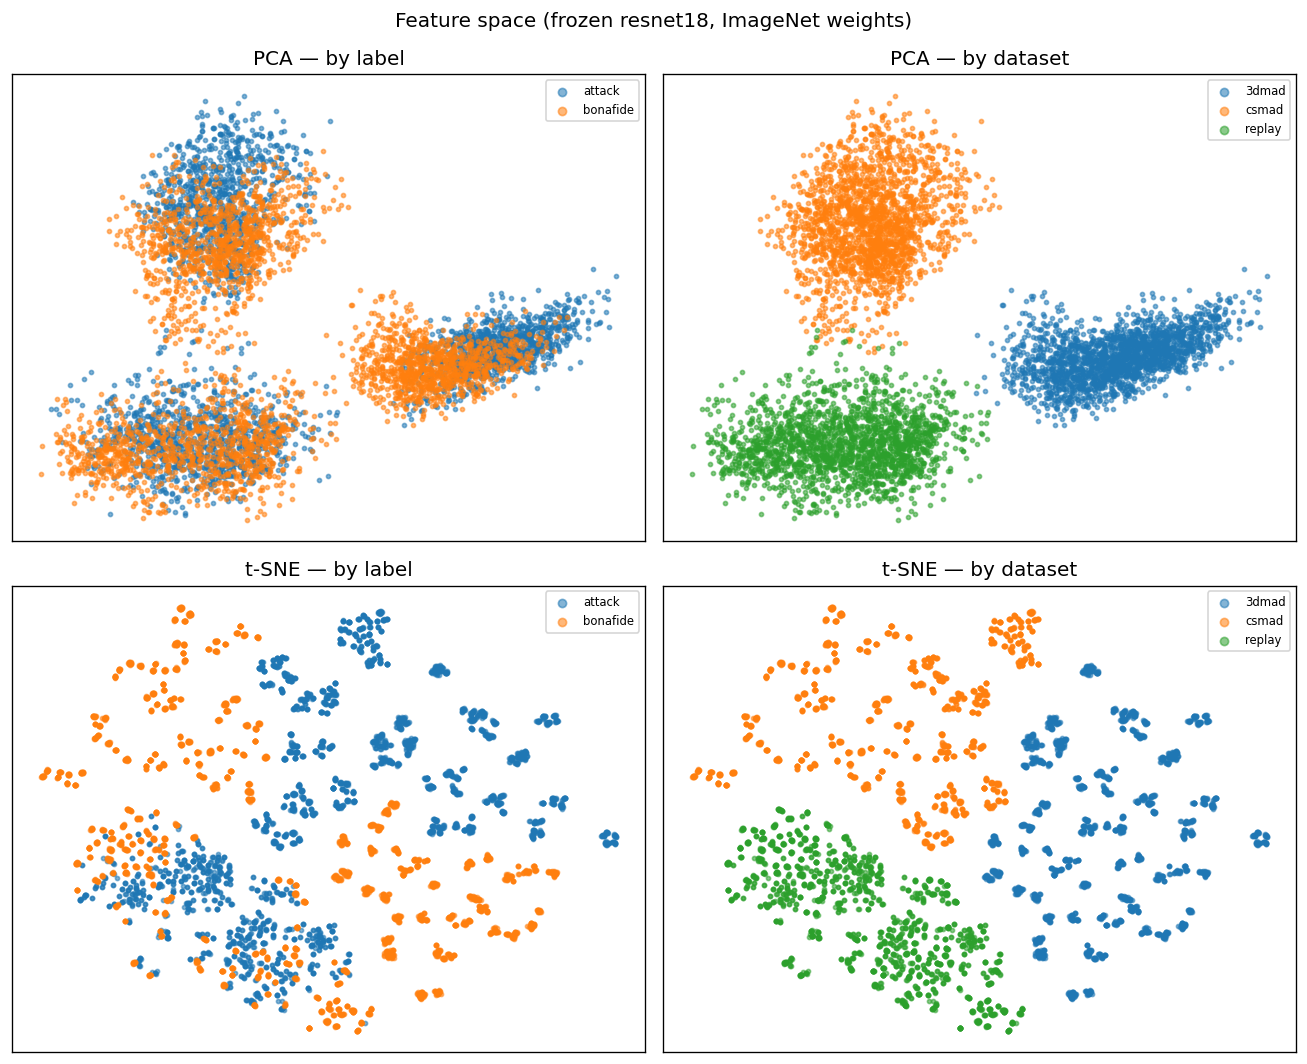
\includegraphics[width=0.92\linewidth]{feature_space.png}
\caption{Frozen ResNet-18 ImageNet features projected with PCA (top)
and t-SNE (bottom). Bonafide vs.\ attack overlap heavily; 3DMAD
vs.\ Replay are visibly separable. The relevant texture cues are not
represented in ImageNet features --- training from scratch is therefore
the right call.}
\label{fig:feature-space}
\end{figure}

\section{Method: AttackNet v2.2}
\label{sec:method}

AttackNet v2.2 is a deliberately small CNN ($8{.}4$M parameters in our
implementation) compared to ResNet-50 ($\sim$$25$M) or VGG-16
($\sim$$138$M). On a constrained domain (single-modality face crops,
$\sim$$10^5$ training images), wider pretrained backbones overfit to
identity and dataset artefacts rather than learning liveness. A
compact model trained from scratch with the right regularisation
performs better in this regime.

\subsection{Architecture}

The network is two residual convolutional blocks followed by a wide
dense head:

\begin{quote}\small
\textbf{Input}: $(B, 3, 256, 256)$ RGB face crop, scaled to $[0,1]$.

\textbf{Block 1} (in$=3$, out$=16$):
$\text{Conv}_{3{\times}3}$, BN, ReLU,
$\text{Conv}_{3{\times}3}$, BN, ReLU, $+\,\text{Conv}_{1{\times}1}$ skip,
$\text{MaxPool}_{2}$, Dropout2d.

\textbf{Block 2} (in$=16$, out$=32$): same shape, channels $16{\to}32$.

\textbf{Head}: Flatten ($\rightarrow 131{,}072$), Linear$\rightarrow 64$, BN,
LeakyReLU($\alpha{=}0{.}2$), Dropout, Linear$\rightarrow 1$ (single logit).
\end{quote}

Three deliberate design choices distinguish v2.2:

\begin{enumerate}[leftmargin=*,topsep=2pt,itemsep=1pt]
\item \textbf{Skip connections add, not concatenate.} Concatenation
   doubles channels and inflates the next conv. Addition keeps channels
   constant at similar accuracy, following the original
   ResNet \cite{he2016resnet} convention.
\item \textbf{LeakyReLU on the dense head.} The flatten-to-$64$
   bottleneck has $\sim$$8.4$M incoming weights; a vanilla ReLU there
   can permanently zero out useful directions early in training (the
   ``dying ReLU'' problem \cite{maas2013leaky}). The leaky variant
   preserves a small gradient through negative activations.
\item \textbf{BatchNorm everywhere.} After every conv and the dense
   bottleneck. Standardising activations across the batch lets us use
   a slightly larger effective learning rate without divergence.
\end{enumerate}

\subsection{Output head and parameter budget}

We use a single linear layer producing one logit per sample, paired
with \texttt{BCEWithLogitsLoss} at training time --- numerically
equivalent to sigmoid + BCE but more stable. The decision boundary is
$\text{logit} = 0$ (equivalently $\sigma(\text{logit})=0{.}5$).

Of the $8{,}406{,}321$ total parameters, $99{.}8\%$ live in the first
dense layer ($131{,}072 \to 64 = 8{,}388{,}672$ weights). This is
typical for a compact-CNN-plus-wide-MLP-head architecture; the
alternative is widening the conv stack, which we have no evidence is
needed at this dataset scale. Memory at inference and training is
modest: peak VRAM at batch $16$ in fp32 is $682$\,MB, leaving a
$12{\times}$ headroom factor on the $8$\,GB GTX 1070.

\subsection{Why train from scratch}

ImageNet pretraining is helpful when the downstream task is semantic
(``cat vs.\ dog''), but liveness detection is largely a texture
classification problem --- moir\'e patterns, paper grain, mask seams.
ImageNet features were learned to \emph{ignore} texture in favour of
semantic content, which is the opposite of what we want.
The EDA result (Section~\ref{sec:eda}, Figure~\ref{fig:feature-space})
confirms this: in frozen ResNet-18 ImageNet features, bonafide and
attack overlap heavily. Training from scratch on liveness data lets
the model build the texture-sensitive filters it actually needs.

\section{Training Protocol}
\label{sec:training}

\subsection{Loss with label smoothing}

We optimise BCE-with-logits against smoothed labels. Given a hard
target $y\in\{0,1\}$ and smoothing $s\!\in\![0,1)$:
\begin{equation}
\tilde y \;=\; y\cdot(1-2s)+s,\qquad
\mathcal{L} \;=\; \text{BCEWithLogits}(\hat y,\,\tilde y).
\end{equation}
We default $s=0.1$. PyTorch's built-in \texttt{label\_smoothing}
argument lives on \texttt{CrossEntropyLoss} and only works for
multiclass distributions, so we apply the smoothing manually.
Smoothing pushes targets away from the saturating regions of the
sigmoid, which improves calibration and helps modestly with
overfitting on a $\sim$$25$k-frame training split. The decision
boundary is unchanged.

\subsection{Optimiser, schedule, augmentation}

\begin{table}[t]
\centering
\caption{Training defaults (\texttt{configs/default.yaml}). Optuna
re-explores LR, dropout, weight decay, batch size, and label smoothing
in Phase~6.}
\label{tab:training-defaults}
\small
\begin{tabular}{l l}
\toprule
Optimiser & Adam \\
Learning rate & $1\!\times\!10^{-6}$ \\
Weight decay & $1\!\times\!10^{-5}$ \\
LR scheduler & ReduceLROnPlateau, factor $0{.}5$, patience $5$, min $10^{-9}$ \\
Early stopping & patience $10$ epochs of no val-ACER improvement \\
Batch size & $16$ \\
Epochs (cap) & $30$ \\
Dropout & $0{.}05$--$0{.}1$ \\
Label smoothing & $0{.}1$ \\
Mixed precision & enabled (\texttt{torch.amp.autocast} + \texttt{GradScaler}) \\
\bottomrule
\end{tabular}
\end{table}

The defaults are listed in Table~\ref{tab:training-defaults}. The
learning rate of $1\!\times\!10^{-6}$ is startlingly small but
defensible: the dense layer dominates the parameter count, and large
LRs blow up its BatchNorm statistics within the first few steps. With
BatchNorm everywhere, internal covariate effects are already mostly
tamed, so the schedule's job is slow refinement rather than fast
descent. Augmentation, applied to the train split only via
Albumentations: rotation $\pm 20^\circ$, horizontal flip ($p\!=\!0{.}5$),
brightness/contrast $\pm 20\%$ ($p\!=\!0{.}5$), Gaussian noise
$\sigma \in [0{.}005,\,0{.}03]$ ($p\!=\!0{.}3$), and motion blur with
kernel up to $5$ ($p\!=\!0{.}3$). We do not apply ImageNet-stat
normalisation --- the network trains from scratch, so plain $[0,1]$
scaling is appropriate.

Mixed precision is enabled by default. On Pascal it halves activation
memory (the conv blocks save $\sim$$250$\,MB at batch $16$), which
matters during Optuna trials when other processes might share the GPU.
If a trial diverges with NaN losses, we disable AMP first with
\texttt{--no-amp} before suspecting other causes.

\subsection{Three protocols, one entry point}

\begin{table}[h]
\centering
\caption{Training protocols. The same training code drives all three
by filtering the manifest on the \texttt{dataset} column.}
\label{tab:protocols}
\small
\begin{tabular}{l l l}
\toprule
\texttt{--protocol} & \texttt{train\_datasets} & \texttt{val\_datasets} \\
\midrule
\texttt{combined} & \{replay, 3dmad\} & \{replay, 3dmad\} \\
\texttt{replay}   & \{replay\}        & \{replay\}        \\
\texttt{3dmad}    & \{3dmad\}         & \{3dmad\}         \\
\bottomrule
\end{tabular}
\end{table}

For zero-shot cross-dataset evaluation we train under one protocol and
evaluate against the held-out dataset's test split.

\subsection{Metrics}

We follow ISO/IEC~30107-3 \cite{iso301073} with the convention
$\text{label}=1\Rightarrow\text{attack}$:
\begin{align}
\text{APCER} &= \tfrac{\#\{\text{attack predicted bonafide}\}}{\#\,\text{attack}}, \\
\text{BPCER} &= \tfrac{\#\{\text{bonafide predicted attack}\}}{\#\,\text{bonafide}}, \\
\text{ACER}  &= \tfrac{1}{2}(\text{APCER}+\text{BPCER}), \\
\text{EER}   &= \text{error at the threshold where APCER}=\text{BPCER}, \\
\text{HTER}  &= \text{ACER at an externally-fixed threshold}.
\end{align}
ACER is the single number we minimise during training (the early-stop
criterion is val-ACER, not val-loss). HTER is the headline
cross-protocol number, and we calibrate its threshold on the target
dataset's devel split before reporting on its test split --- an honest
protocol that does not peek at test labels.

We additionally report \emph{video-level} numbers: per-video
probabilities are obtained by averaging frame probabilities over a
\texttt{source\_video}, then re-thresholded. This reduces frame-wise
noise and is the standard headline reporting style for video-based
liveness benchmarks.

\subsection{Cross-validation}

To complement the official train/devel/test partition we additionally
run $5$-fold subject-disjoint cross-validation. Folds are constructed
so that all frames from a given subject stay together. This rules out
the most common information leak in PAD experiments, where the same
person appears in both training and validation under different attack
conditions. The CV results are computed on the train+devel union; the
test split is held out for the final reporting in
Section~\ref{sec:within-dataset}.

\section{Experiments}
\label{sec:experiments}

We report three blocks of results: $5$-fold subject-disjoint
cross-validation (Section~\ref{sec:cv}), held-out test-set evaluation
in the within-dataset regime (Section~\ref{sec:within-dataset}), and
zero-shot cross-dataset evaluation under both fixed and devel-calibrated
thresholds (Section~\ref{sec:cross-dataset}).

\subsection{Cross-validation results}
\label{sec:cv}

\begin{table}[h]
\centering
\caption{$5$-fold subject-disjoint cross-validation, mean $\pm$ std
over folds, on the validation portion of each fold (frame-level).}
\label{tab:cv}
\small
\begin{tabular}{l c c c c c}
\toprule
Protocol & ACER & APCER & BPCER & EER & ROC-AUC \\
\midrule
Combined & $0{.}0022\!\pm\!0{.}0019$ & $0{.}0040\!\pm\!0{.}0040$ & $0{.}0004\!\pm\!0{.}0006$ & $0{.}0025\!\pm\!0{.}0023$ & $0{.}9999\!\pm\!0{.}0002$ \\
Replay   & $0{.}0023\!\pm\!0{.}0036$ & $0{.}0030\!\pm\!0{.}0043$ & $0{.}0016\!\pm\!0{.}0028$ & $0{.}0022\!\pm\!0{.}0036$ & $0{.}9998\!\pm\!0{.}0002$ \\
3DMAD    & $0{.}0028\!\pm\!0{.}0057$ & $0{.}0000\!\pm\!0{.}0000$ & $0{.}0057\!\pm\!0{.}0113$ & $0{.}0000\!\pm\!0{.}0000$ & $1{.}0000\!\pm\!0{.}0000$ \\
\bottomrule
\end{tabular}
\end{table}

Table~\ref{tab:cv} reports CV numbers. All three protocols sit below
$0{.}3\%$ ACER and above $0{.}9998$ ROC-AUC. The fold-spread is
visualised in Figure~\ref{fig:cv-fold-spread}: 3DMAD has the highest
variance across folds because each fold rotates a small number of
subjects out, which can sway error rates non-trivially when the
subject pool is only $17$ people.

Mean early-stopping epochs per protocol --- combined $\sim$$28$,
Replay $\sim$$36$, 3DMAD $\sim$$12$ --- match the intuitive ordering:
3DMAD converges fastest because it is smaller and its single attack
type is the easiest to learn, and combined training takes longest
because the model must reconcile two different domains. We
interpret the larger combined-protocol training time as evidence that
combined training is doing real learning work, not merely averaging
two single-domain models.

\begin{figure}[h]
\centering
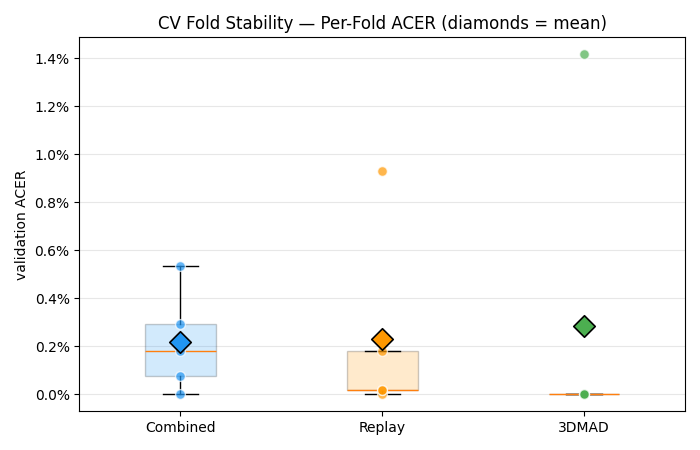
\includegraphics[width=0.85\linewidth]{cv_fold_spread.png}
\caption{Per-fold ACER. 3DMAD's higher fold-to-fold variance reflects
the small subject pool (only 17 people).}
\label{fig:cv-fold-spread}
\end{figure}

\subsection{Within-dataset test-set evaluation}
\label{sec:within-dataset}

\begin{table}[h]
\centering
\caption{Held-out test-set evaluation, frame- and video-level. Each
model is the best-fold checkpoint of its protocol. The test split was
not seen during training or cross-validation.}
\label{tab:within}
\small
\begin{tabular}{l c c c c c}
\toprule
Protocol & ACER & APCER & BPCER & EER & ROC-AUC \\
\midrule
\multicolumn{6}{l}{\emph{Frame level}} \\
Combined & $0{.}0037$ & $0{.}0001$ & $0{.}0073$ & $0{.}0012$ & $1{.}0000$ \\
Replay   & $0{.}0007$ & $0{.}0014$ & $0{.}0000$ & $0{.}0004$ & $1{.}0000$ \\
3DMAD    & $0{.}0015$ & $0{.}0000$ & $0{.}0030$ & $0{.}0000$ & $1{.}0000$ \\
\midrule
\multicolumn{6}{l}{\emph{Video level (per-video probability mean)}} \\
Combined & $0{.}0038$ & $0{.}0000$ & $0{.}0077$ & $0{.}0000$ & $1{.}0000$ \\
Replay   & $0{.}0000$ & $0{.}0000$ & $0{.}0000$ & $0{.}0000$ & $1{.}0000$ \\
3DMAD    & $0{.}0000$ & $0{.}0000$ & $0{.}0000$ & $0{.}0000$ & $1{.}0000$ \\
\bottomrule
\end{tabular}
\end{table}

\begin{figure}[h]
\centering
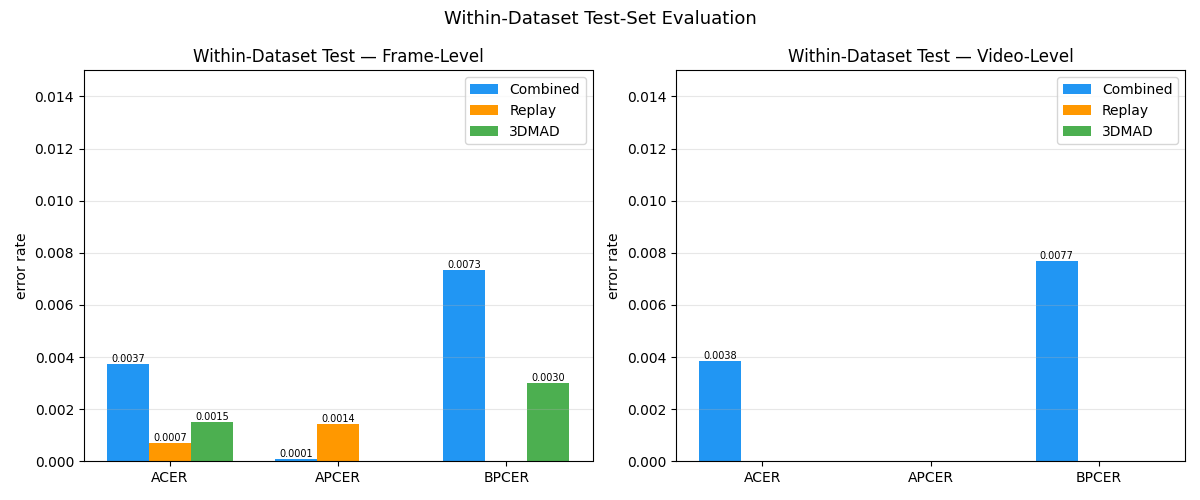
\includegraphics[width=0.85\linewidth]{within_dataset_bars.png}
\caption{Within-dataset test ACER (bars) and APCER/BPCER decomposition.
All three protocols are sub-$0{.}5\%$. The combined model is slightly
behind the single-dataset models on each domain but covers both.}
\label{fig:within-bars}
\end{figure}

All three protocols achieve near-perfect within-dataset separation
(Table~\ref{tab:within}, Figure~\ref{fig:within-bars}). At the
frame level, the single-dataset models slightly outperform the
combined model on their own test set --- they only need to learn one
domain's characteristics --- but the gap is $\le 0{.}3\%$ ACER. At the
video level the per-video probability average drives the
single-dataset models to $0{.}0000$ ACER and pulls combined to
$0{.}0038$. We do not over-interpret these numbers; both Replay-Attack
and 3DMAD are widely regarded as ``solved'' by modern standards, and
the more interesting comparison is the cross-dataset behaviour below.

\subsection{Cross-dataset evaluation}
\label{sec:cross-dataset}

\begin{table}[h]
\centering
\caption{Zero-shot cross-dataset evaluation, fixed threshold $0{.}5$.}
\label{tab:cross-fixed}
\small
\begin{tabular}{l c c c c}
\toprule
Direction & Frame ACER & Frame APCER & Frame BPCER & Video ACER \\
\midrule
Replay $\rightarrow$ 3DMAD & $0{.}0280$ & $0{.}0407$ & $0{.}0153$ & $0{.}0300$ \\
3DMAD  $\rightarrow$ Replay & $0{.}3875$ & $0{.}7511$ & $0{.}0238$ & $0{.}3975$ \\
\bottomrule
\end{tabular}
\end{table}

\begin{table}[h]
\centering
\caption{Zero-shot cross-dataset HTER, threshold calibrated on the
target dataset's devel split before reporting on its test split.}
\label{tab:cross-hter}
\small
\begin{tabular}{l c c c c}
\toprule
Direction & Threshold & Test HTER & APCER & BPCER \\
\midrule
Replay $\rightarrow$ 3DMAD & $0{.}6442$ & $0{.}0883$ & $0{.}1767$ & $0{.}0000$ \\
3DMAD  $\rightarrow$ Replay & $0{.}3030$ & $0{.}2267$ & $0{.}2791$ & $0{.}1742$ \\
\bottomrule
\end{tabular}
\end{table}

\begin{figure}[h]
\centering
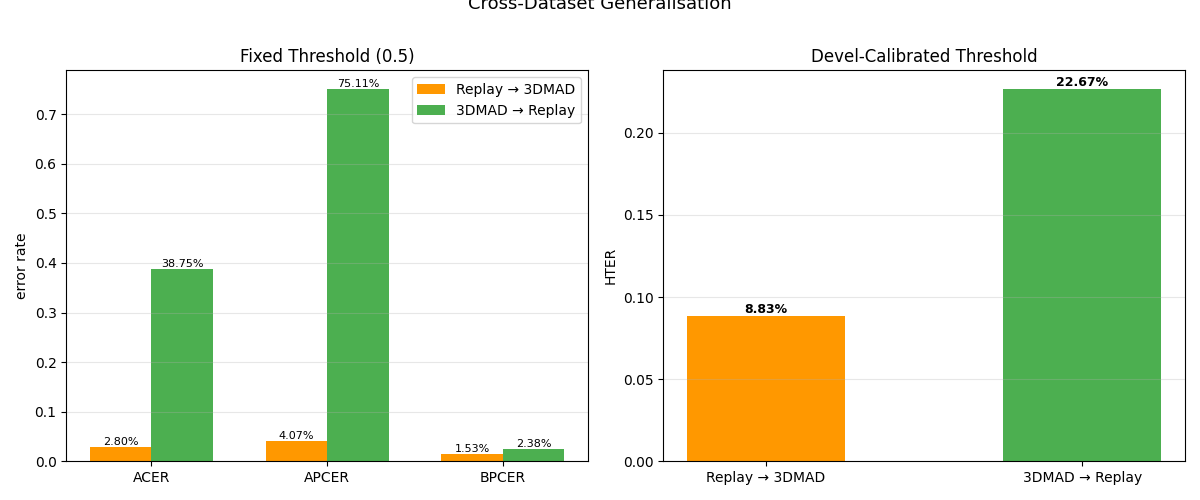
\includegraphics[width=0.85\linewidth]{cross_dataset_bars.png}
\caption{Zero-shot cross-dataset error rates at the fixed-$0{.}5$
threshold. The asymmetry is the headline finding: Replay
$\rightarrow$ 3DMAD transfers; 3DMAD $\rightarrow$ Replay does not.}
\label{fig:cross-bars}
\end{figure}

\begin{table}[h]
\centering
\caption{Combined $\rightarrow$ CSMAD, devel-calibrated HTER.
Threshold set at devel EER; HTER reported on test.
devel: $n{=}7{,}347$ (subjects C, D, J, K);
test: $n{=}6{,}027$ (subjects E, F, L, M, N).}
\label{tab:cross-csmad}
\small
\begin{tabular}{l c c c c c}
\toprule
Direction & Threshold & HTER & APCER & BPCER & AUC \\
\midrule
Combined $\rightarrow$ CSMAD & $0{.}9071$ & $0{.}5807$ & $0{.}4669$ & $0{.}6945$ & $0{.}4012$ \\
\bottomrule
\end{tabular}
\end{table}

Table~\ref{tab:cross-csmad} shows the most severe failure mode in
this study. The HTER of $0{.}58$ is worse than a coin flip ($0{.}5$),
but the decisive number is the ROC-AUC of $\mathbf{0{.}40}$. An AUC
below $0{.}5$ is a \emph{ranking inversion}: the model assigns higher
attack scores to bonafide CSMAD faces than to silicon masks. This is
not a threshold artefact --- it persists even after calibration on the
devel split. The calibrated threshold of $0{.}907$ reveals the
underlying bias: the model assigns high attack probability to almost
everything in the CSMAD domain, but genuine faces score even higher
than attacks.

The mechanism differs from the Replay/3DMAD cross-dataset failures.
There, the model simply lacked features that fire on the unseen attack
type. Here, the RealSense SR300's sensor characteristics --- noise
floor, dynamic range, IR bleed --- push \emph{real} faces into the
high-attack region of the learned feature space. Silicon masks,
as high-quality physical objects under controlled lab lighting,
produce images that more closely resemble the training distribution's
bonafide class. The domain shift affects real faces more severely than
it affects the attacks, which inverts the ranking.

The cross-dataset numbers (Tables~\ref{tab:cross-fixed} and
\ref{tab:cross-hter}, Figure~\ref{fig:cross-bars}) for Replay/3DMAD
tell the same story at a smaller scale. Replay $\rightarrow$ 3DMAD is workable: at the fixed threshold
of $0{.}5$, frame ACER is $2{.}80\%$, and devel-calibrated HTER on
the 3DMAD test split is $8{.}83\%$. 3DMAD $\rightarrow$ Replay
collapses: $38{.}75\%$ frame ACER at fixed threshold, and even after
devel calibration the HTER is $22{.}67\%$. The APCER decomposition
makes the failure mode unambiguous: a 3DMAD-only model classifies
$75\%$ of Replay attacks as bonafide. It has not learned ``liveness''
in any general sense; it has learned a narrow boundary specific to
3D-mask vs.\ Kinect-RGB-real.

\section{Discussion}
\label{sec:discussion}

\textbf{The asymmetry is the finding.} A model trained on
Replay-Attack's diverse 2D presentations (print, mobile, high-def,
video; 50 subjects; both controlled and adverse lighting) carries
some of that diversity into the cross-dataset regime. A model trained
on 3DMAD's single attack type ($17$ subjects, one lighting condition,
one camera, one mask family) has a brittle decision surface that does
not transfer. The takeaway is not that Replay is a ``better'' dataset
in the abstract --- it is that \emph{training-data diversity matters
more than training-set size}. Replay has $4\times$ fewer subjects than
a real-world deployment would have, but its $5$ attack types give the
model enough signal to partially generalise; 3DMAD's single attack type
produces a model that does not know what a 2D presentation even looks
like.

\textbf{Combined training is the minimum viable strategy.} The
combined model achieves $0{.}22\%$ CV ACER and $0{.}37\%$ test ACER on
the union of the two domains, while being exposed to both 2D and 3D
attacks. It does not sacrifice within-domain accuracy for breadth ---
the gap between the combined model and the best single-dataset model
on its own domain is sub-$0{.}3\%$ at the frame level, and zero at the
video level for the single-dataset models. We read this as evidence
that the cost of merging benchmarks is essentially nil; the
benefit is the entire cross-dataset gap.

\textbf{Near-zero within-dataset error is not real-world readiness.}
Both Replay-Attack and 3DMAD have small subject pools, fixed cameras,
and limited backgrounds. The cross-dataset asymmetry shows that even
``saturated'' benchmarks have substantial residual error when one
goes off-distribution, and any production system will operate
off-distribution by definition.

\textbf{Limitations.} (i) We use only RGB. A multi-modal pipeline that
exploits 3DMAD's depth or CSMAD's IR/thermal streams would change the
problem and would likely change the cross-dataset numbers. We chose
RGB-only deliberately because it is the harder problem and matches
the deployment constraint of consumer phones. (ii) We use a single
detector (RetinaFace via \texttt{insightface buffalo\_sc}) and accept
the small fraction of dropped frames where it returns no
detection ($4$ frames out of $61{,}996$ on Replay; $0$ on 3DMAD).
This is unlikely to materially affect any number we report, but a
production pipeline would need a fallback. (iii) The hardware budget
(GTX 1070, 8\,GB VRAM) bounds the architecture and the augmentation
schedule. A larger model, a wider augmentation schedule, or domain
adaptation might close the cross-dataset gap further.

\section{CSMAD Out-of-Distribution Probe}
\label{sec:csmad}

\subsection{Setup}

CSMAD (Custom Silicone Mask Attack Database) ships HDF5 captures from
an Intel RealSense SR300 (RGB, NIR, depth) and a Seek thermal camera,
with $87$ bonafide videos and $159$ attack videos in two pose families
(\texttt{WEAR} and \texttt{STAND}); we use only the SR300
\texttt{color} channel. Each frame is a separate timestamped dataset
of shape $(H,W,3)$ \texttt{uint8} under \texttt{data/sr300/color}.
The extractor lists keys, sorts them chronologically, and steps
through with \texttt{FRAME\_STRIDE=5}, exactly as for the other
datasets. The extractor handles two naming conventions across
WEAR/STAND subfolders: \texttt{\{camera\}\_atk\_\{wearer\}\{mask\}\_...h5}
(WEAR) and \texttt{Mask\_atk\_\{wearer\}\{mask\}\_...h5} (STAND).
After extraction, CSMAD contributes $18{,}763$ frames across $243$
videos.

CSMAD is held out entirely from training. The attack archive only
covers subjects A--F; distributing those six subjects across all three
partitions gives attacks in every split:

\begin{center}\small
\begin{tabular}{l l r r}
\toprule
Split & Subjects & Bonafide & Attack \\
\midrule
train & A, B, G, H, I & $1{,}017$ & $4{,}372$ \\
devel & C, D, J, K    & $1{,}449$ & $5{,}898$ \\
test  & E, F, L, M, N & $1{,}679$ & $4{,}348$ \\
\bottomrule
\end{tabular}
\end{center}

\subsection{Results and interpretation}

We evaluate the combined model (\texttt{both-cv-5/fold\_1/best.pt})
using the devel-calibrated HTER protocol (threshold set at devel EER,
reported on test). Results are in Table~\ref{tab:cross-csmad}.

The headline number is the AUC of $\mathbf{0{.}40}$ --- a ranking
inversion. The model assigns higher attack scores to bonafide CSMAD
faces than to silicon masks. This is not a threshold artefact: after
calibration on devel, the threshold rises to $0{.}907$ (far above the
default $0{.}5$) yet the HTER is still $0{.}58$, worse than random.

The inversion mechanism differs from the Replay/3DMAD cross-dataset
failures. There, the model lacked features that fire on the unseen
attack type. Here, the RealSense SR300 sensor's characteristics ---
noise floor, dynamic range, IR bleed into the colour channel ---
produce real-face images that land in the high-attack region of the
learned feature space. Silicon masks, as high-quality physical objects
under controlled lab lighting, produce images closer to the training
distribution's bonafide class. The domain shift hurts real faces more
than it hurts the attacks, which inverts the ranking entirely.

This result sharpens the cross-dataset conclusion: the failure is not
about attack-type novelty but about sensor novelty. An RGB-only PAD
model trained on fixed-camera benchmarks does not generalise to new
capture hardware, and the failure mode when it encounters one can be
worse than random --- a fact invisible from within-dataset evaluation
alone.

\section{Conclusion}
\label{sec:conclusion}

We presented a unified RGB preprocessing pipeline that ingests two
structurally different public benchmarks --- Replay-Attack and 3DMAD
--- into a single CSV manifest of $77{,}296$ uniformly cropped
$256{\times}256$ face images, and trained a compact $8{.}4$M-parameter
residual CNN (AttackNet v2.2) from scratch on their union.
Within-dataset test ACER is below $0{.}5\%$ on both benchmarks.

Cross-dataset evaluation reveals a sharp asymmetry: Replay
$\rightarrow$ 3DMAD transfers at $2{.}8\%$ frame ACER (devel-calibrated
HTER $8{.}8\%$), while 3DMAD $\rightarrow$ Replay collapses to
$38{.}8\%$ (HTER $22{.}7\%$). The asymmetry is evidence that
single-dataset models learn camera- and protocol-specific shortcuts
rather than a general notion of liveness. Combined training closes
most of this gap at negligible within-domain cost.

A devel-calibrated probe on the entirely held-out CSMAD corpus
(silicone mask attacks, Intel RealSense SR300) produces the sharpest
finding: HTER $0{.}58$ and ROC-AUC $0{.}40$ --- a \emph{ranking
inversion}. The combined model assigns higher attack scores to
genuine CSMAD faces than to silicon masks. The cause is sensor
domain shift, not attack-type novelty: the SR300's noise and
dynamic range characteristics push real faces into the high-attack
region of the learned feature space while masks remain near the
boundary. AUC below $0{.}5$, confirmed after threshold calibration,
is the empirical signature. The practical implication: a PAD model
that saturates a fixed-camera benchmark can perform worse than
random on a new camera, with real users rejected more aggressively
than attackers --- a risk entirely invisible from within-dataset
evaluation alone.

\section*{Acknowledgements}
The authors thank the maintainers of the Replay-Attack and 3DMAD
benchmarks for making their data publicly available, and the
\texttt{insightface} project for the \texttt{buffalo\_sc} face
detector.

\begin{thebibliography}{99}

\bibitem{anjos2011replay}
A.~Anjos and S.~Marcel.
\newblock Counter-measures to photo attacks in face recognition: a public
  database and a baseline.
\newblock In \emph{Int.\ Joint Conf.\ on Biometrics (IJCB)}, 2011.

\bibitem{erdogmus20143dmad}
N.~Erdogmus and S.~Marcel.
\newblock Spoofing face recognition with 3D masks.
\newblock \emph{IEEE Trans.\ Information Forensics and Security}, 9(7):1084--1097, 2014.

\bibitem{bhattacharjee2018csmad}
S.~Bhattacharjee, A.~Mohammadi, and S.~Marcel.
\newblock Spoofing deep face recognition with custom silicone masks.
\newblock In \emph{IEEE Int.\ Conf.\ on Biometrics: Theory, Applications and Systems (BTAS)}, 2018.

\bibitem{he2016resnet}
K.~He, X.~Zhang, S.~Ren, and J.~Sun.
\newblock Deep residual learning for image recognition.
\newblock In \emph{CVPR}, 2016.

\bibitem{ioffe2015batchnorm}
S.~Ioffe and C.~Szegedy.
\newblock Batch normalization: accelerating deep network training by
  reducing internal covariate shift.
\newblock In \emph{ICML}, 2015.

\bibitem{maas2013leaky}
A.~L. Maas, A.~Y. Hannun, and A.~Y. Ng.
\newblock Rectifier nonlinearities improve neural network acoustic models.
\newblock In \emph{ICML Workshop on Deep Learning for Audio, Speech and Language Processing}, 2013.

\bibitem{he2015kaiming}
K.~He, X.~Zhang, S.~Ren, and J.~Sun.
\newblock Delving deep into rectifiers: surpassing human-level performance
  on ImageNet classification.
\newblock In \emph{ICCV}, 2015.

\bibitem{kingma2014adam}
D.~P. Kingma and J.~Ba.
\newblock Adam: a method for stochastic optimization.
\newblock \emph{arXiv preprint arXiv:1412.6980}, 2014.

\bibitem{iso301073}
ISO/IEC 30107-3:2017.
\newblock Information technology -- biometric presentation attack
  detection -- Part 3: testing and reporting.
\newblock International Organization for Standardization, 2017.

\end{thebibliography}

\end{document}
